\documentclass[12pt]{article}

\usepackage{tgtermes}
\usepackage{epsf}
\usepackage{epstopdf}
\usepackage{amsmath}
\usepackage{graphicx}
\usepackage{booktabs}
\usepackage[colorlinks=true,linkcolor=blue,citecolor=blue]{hyperref}
\usepackage{dcolumn}
\usepackage{amsmath, amsthm, amssymb}
\usepackage{mwe}
\usepackage{url}
%\usepackage{harvard}
\usepackage{fancyheadings}
\usepackage{longtable}
\usepackage{authblk}
\usepackage{setspace}
%\usepackage[nomarkers]{endfloat}
\usepackage{float}
\usepackage{bbm}
%\usepackage{titling}
\usepackage{subcaption}
\usepackage{algorithm}
\usepackage{algorithmic}
\usepackage{import}
\usepackage[backend=biber,style=authoryear,
sorting=ynt,citestyle=authoryear]{biblatex}
\addbibresource{papercitations.bib}
%\usepackage[nomarkers,nofiglist,notablist]{endfloat}
\usepackage{subcaption}
\usepackage{caption}

\onehalfspacing
\textwidth 6.5in \oddsidemargin 0in \evensidemargin -0.6in
\textheight 8.5in \topmargin -0.2in

\newcolumntype{L}[1]{>{\raggedright\let\newline\\
		\arraybackslash\hspace{0pt}}m{#1}}
\newcolumntype{C}[1]{>{\centering\let\newline\\
		\arraybackslash\hspace{0pt}}m{#1}}
\newcolumntype{R}[1]{>{\raggedleft\let\newline\\
		\arraybackslash\hspace{0pt}}m{#1}}
\newcolumntype{P}[1]{>{\raggedright\tabularxbackslash}p{#1}}

\newtheorem{theorem}{Theorem}[section]
\newtheorem{corollary}[theorem]{Corollary}
\newtheorem{proposition}[theorem]{Proposition}
\newtheorem{lemma}[theorem]{Lemma}

\captionsetup{justification=centering,singlelinecheck=false}


\newcommand{\xsub}[1]{%
	\mbox{\scriptsize\begin{tabular}{@{}c@{}}#1\end{tabular}}%
}

%\renewcommand{\thetable}{\Roman{table}}

\begin{document}
	
	
	
	
	\linespread{1.2}\title{\vspace{-0.5in} Common Ownership in the Nonprofit Sector:\newline Evidence from the Hospital Industry} 
	
	\date{\today}
	
	\author{\vspace{10mm}Hanna Glenn\footnote{Department of Economics, Emory University, 1602 Fishburne Drive, Atlanta, GA 30322, hanna.glenn@emory.edu.} }
	
	\maketitle
	%\setlength{\droptitle}{-10pt}
	
	\vspace{-0.2in}
	
	\singlespacing\maketitle


 \vspace{3mm}
	
    \begin{abstract}
		{\small

		} 
	\end{abstract}
	
	
	
	
	

	
	\onehalfspacing
	
	\newpage

    \section{Introduction}

    Several concerns arise when firms in direct competition share affiliated ownership. One example is common ownership, where investors hold substantial shares of firms in the same industry. While such investors do not actively manage the firms they own, they exert influence over firm behavior through voting rights and shareholder meetings. The common ownership hypothesis, first introduced by \citeauthor{rotemberg1984financial} (\citeyear{rotemberg1984financial}), posits that profit-maximizing firms place nonzero weight on the profits of competitors with shared owners. This raises antitrust concerns, as it may facilitate indirect collusion, affecting competition and prices. In this paper, I examine whether nonprofit firm behavior exhibits similar patterns of affiliation-driven influence.

    Unlike public firms, nonprofits do not have shareholders. Instead, they are guided by a board of directors: a group of volunteers responsible for selecting executives and holding them accountable. In some ways, a board functions similarly to shareholders, they influence the strategic direction of the organization without actively managing day-to-day operations. As with common ownership, there are no legal restrictions preventing directors from serving on multiple boards, even if those firms are competing. Therefore, if the firms are profit-maximizing and the board of directors influence the profit function, a parallel to the common ownership hypothesis arises. While previous studies have documented increased prices under common ownership in industries such as airlines and banking (\cite{azar2018anticompetitive}; \cite{azar2022ultimate}), no research has examined this phenomenon in the nonprofit sector. 
    
    The purpose of this paper is two-fold. First, I document the extent of board-level affiliation among plausibly independent nonprofit hospitals, capturing a nonprofit equivalent to common ownership. Second, I explore the potential competitive effects of board affiliations on hospital behavior. The hospital industry provides an ideal setting for this study for three reasons. First, nonprofit hospitals play a dominant role in US health care. As of 2023, 50\% of hospitals were private nonprofits, compared to 36\% for-profit. Moreover, nonprofit hospitals operate larger facilities, with an average of 207 staffed beds, compared to 107 in for-profits (\cite{ASPE_2023}). Therefore, nonprofit hospital behavior directly impacts the patient population in the US. Second, nonprofit hospitals are often suspected of behaving like "for-profits in disguise" (citation needed), making them an appropriate context for testing the common ownership hypothesis, which assumes firms are profit-driven. Finally, hospital mergers and consolidations are under increasing scrutiny as competition in the sector has declined significantly in recent years (add cite). 

    I compile information on hospital board of director teams from publicly available Tax Form 990s, filed each year by nonprofits in the US. One section of this form requires declaration of the names of each member of the board, executives, and highest compensated employees. Extracting these identities and matching to other sources of hospital information, I form a network of hospital board members from 2017-2022. I show that nearly 10\% of the nonprofit hospitals in the sample are affiliated with another hospital by board, even excluding any system or network affiliations. Two-thirds of affiliated pairs are made up of two general hospitals, with the remaining pairs consisting of a general hospital affiliated with a specialty hospital. 



    \section{Documenting Board of Director Affiliation}

    I compile data on nonprofit hospital board of directors from publicly available Tax Form 990s, which most nonprofits in the US complete each year. These forms contain a section in which firms declare their board, executives, and highest compensated employees. I limit to firms that have a completed Schedule H in the 990, indicating that the firm runs a hospital. PDF version of the 990s are made public by Nonprofit Explorer dating back earlier than 2009. However, using OCR text extraction on non-readable PDFs is both time consuming and potentially inaccurate. Thus, I analyze the data from 2017 onward, when the IRS began publishing XML versions of these files. 

    Extracting the relevant names from the XML files, this data yields a list of names and associated titles for each hospital, year observation. I clean the name column by removing common titles such as Dr., Reverand, etc. and combining names within the same firm that have slight spelling differences. For example, if John Matthews is a board member of hospital A in 2016, and John Mathews is a board member of hospital B in 2017, I combine these to be the same person. Additionally, I combine names within the same HRR that are identical apart from small mischaracters such as the presence of a middle initial. Finally, to avoid issues in whether first or last names are listed first, I sort each individual's names alphabetically. 

    There are several requirements for two hospitals to be affiliated through board members. First, and most relevant, there must be at least one shared board member on each hospital's board of directors. Second, hospitals must be within the same market to be considered affiliated by board member. For these purposes, I define a market as a Hospital Referral Region (HRR), defined by (fill in details here). I focus on markets since the outcomes of interest capture changes in competative behavior, which is most salient within the same market. Furthermore, it is much less likely for two different hospital board members in the same HRR to share an identical name. Finally, I focus on affiliations that are not due to being in the same system or network. Whether the hospital is independent or part of a system, I only consider board connections with hospitals that are independent or associated with a separate hospital system. Of the (blank) hospitals in the sample, almost 10\% are affiliated with another hospital through a shared board member. As shown in Figure \ref{fig:connected_percent}, this percentage remains constant over time. 

    \begin{figure}[ht!]
        \centering
        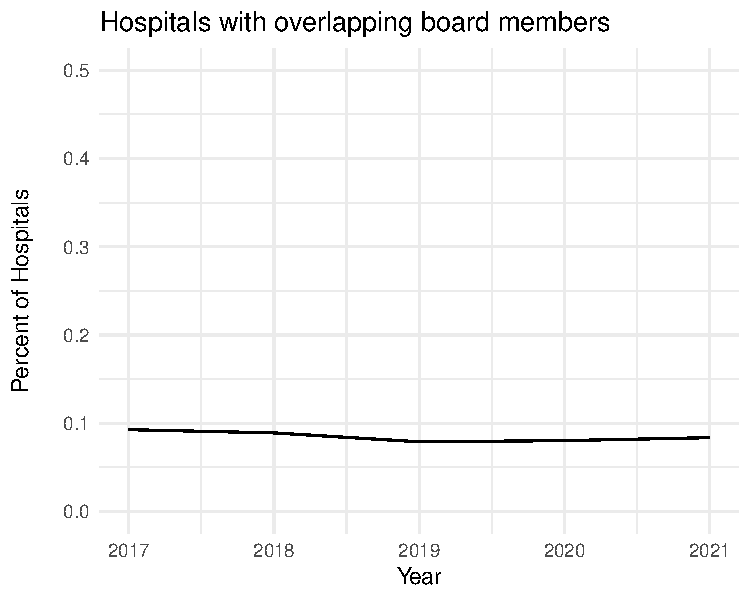
\includegraphics[width=.7\textwidth]{Objects/connected_percent.pdf}
        \label{fig:connected_percent}
    \end{figure}

    As mentioned previously, common board members should be the most prominent within a hospital market, where hospitals compete for the same patient population. Of the (blank) HRRs in the US, approximately 17\% have at least one pair of connected hospitals within the market. As shown in Figure \ref{fig:connected_HRR_percent}, this proportion decreases slightly over time, with 15\% of HRRs having connected hospitals in 2021.  

    \begin{figure}[ht!]
        \centering
        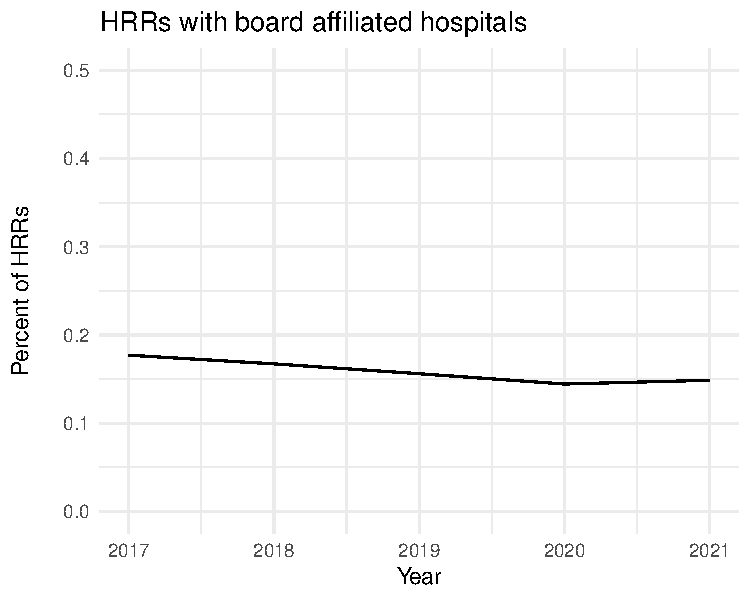
\includegraphics[width=.7\textwidth]{Objects/connected_independent_HRR_percent.pdf}
        \label{fig:connected_HRR_percent}
    \end{figure}

    The geographic distribution of these pairs is shown in Figure \ref{fig:connected_maps}, where the blue dots represent hospitals that share a common board member. Connected hospitals are distributed fairly regularly across the US, apart from relatively few connections on the west coast relative to the population. 

    \begin{figure}[ht!]
        \centering
        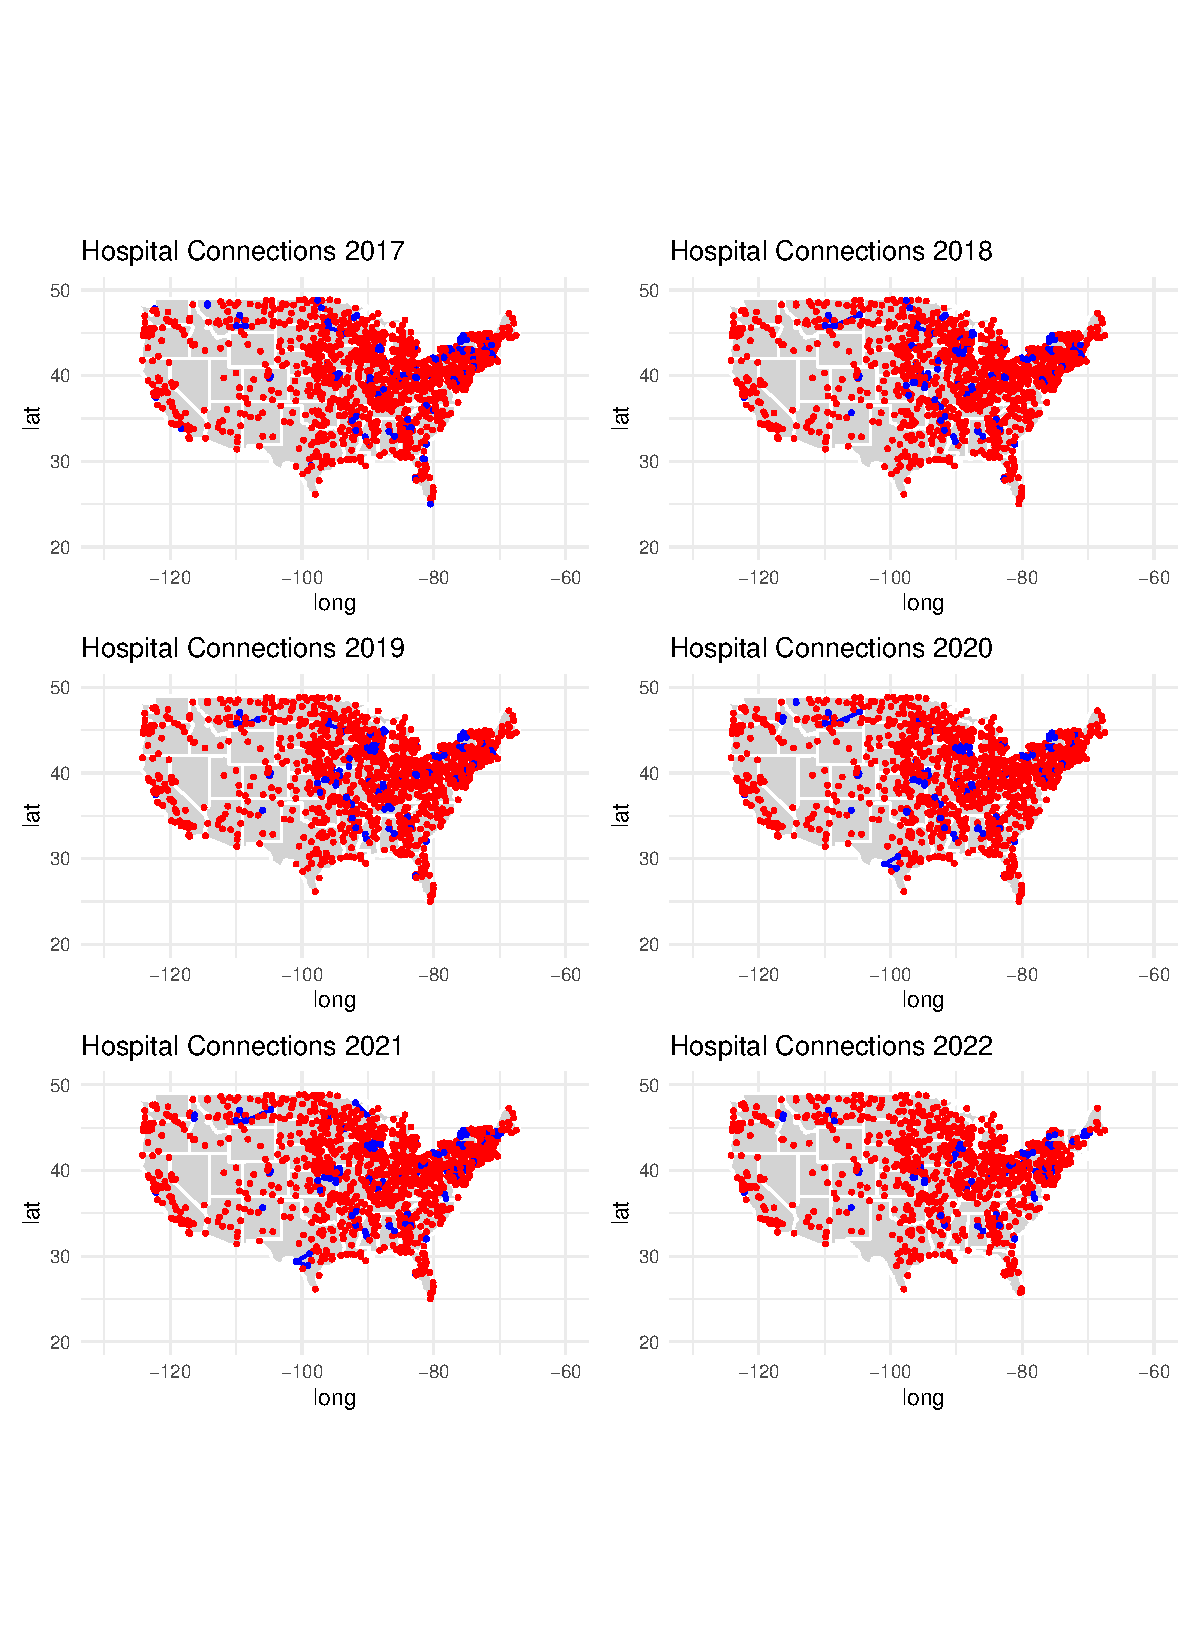
\includegraphics[width=\textwidth]{Objects/connected_maps.pdf}
        \label{fig:connected_maps}
    \end{figure}

    Finally, I show the proportion of hospital pairs broken down by type. Each hospital can be general or specialty, children or adult, and independent or system. In Table \ref{tab:hospital_pair_types}, I show that the majority of pairs are both general hospitals, and that there is significant variation in the ownership type of pairs. Forty-five percent of pairs are between two non-system affiliated hospitals, and 36\% of pairs are between an independent hospital affiliated with a hospital belonging to a system. 

    \import{Objects}{hospital_pair_types.tex}


    \section{Does Board Affiliation Matter for Competition?}

    \import{Objects}{hospital_connected_summary.tex}

    


    

    

    

    

    

	
	
	


\end{document}

